\subsection{Loci of the Brocard points}

\begin{figure}
    \centering
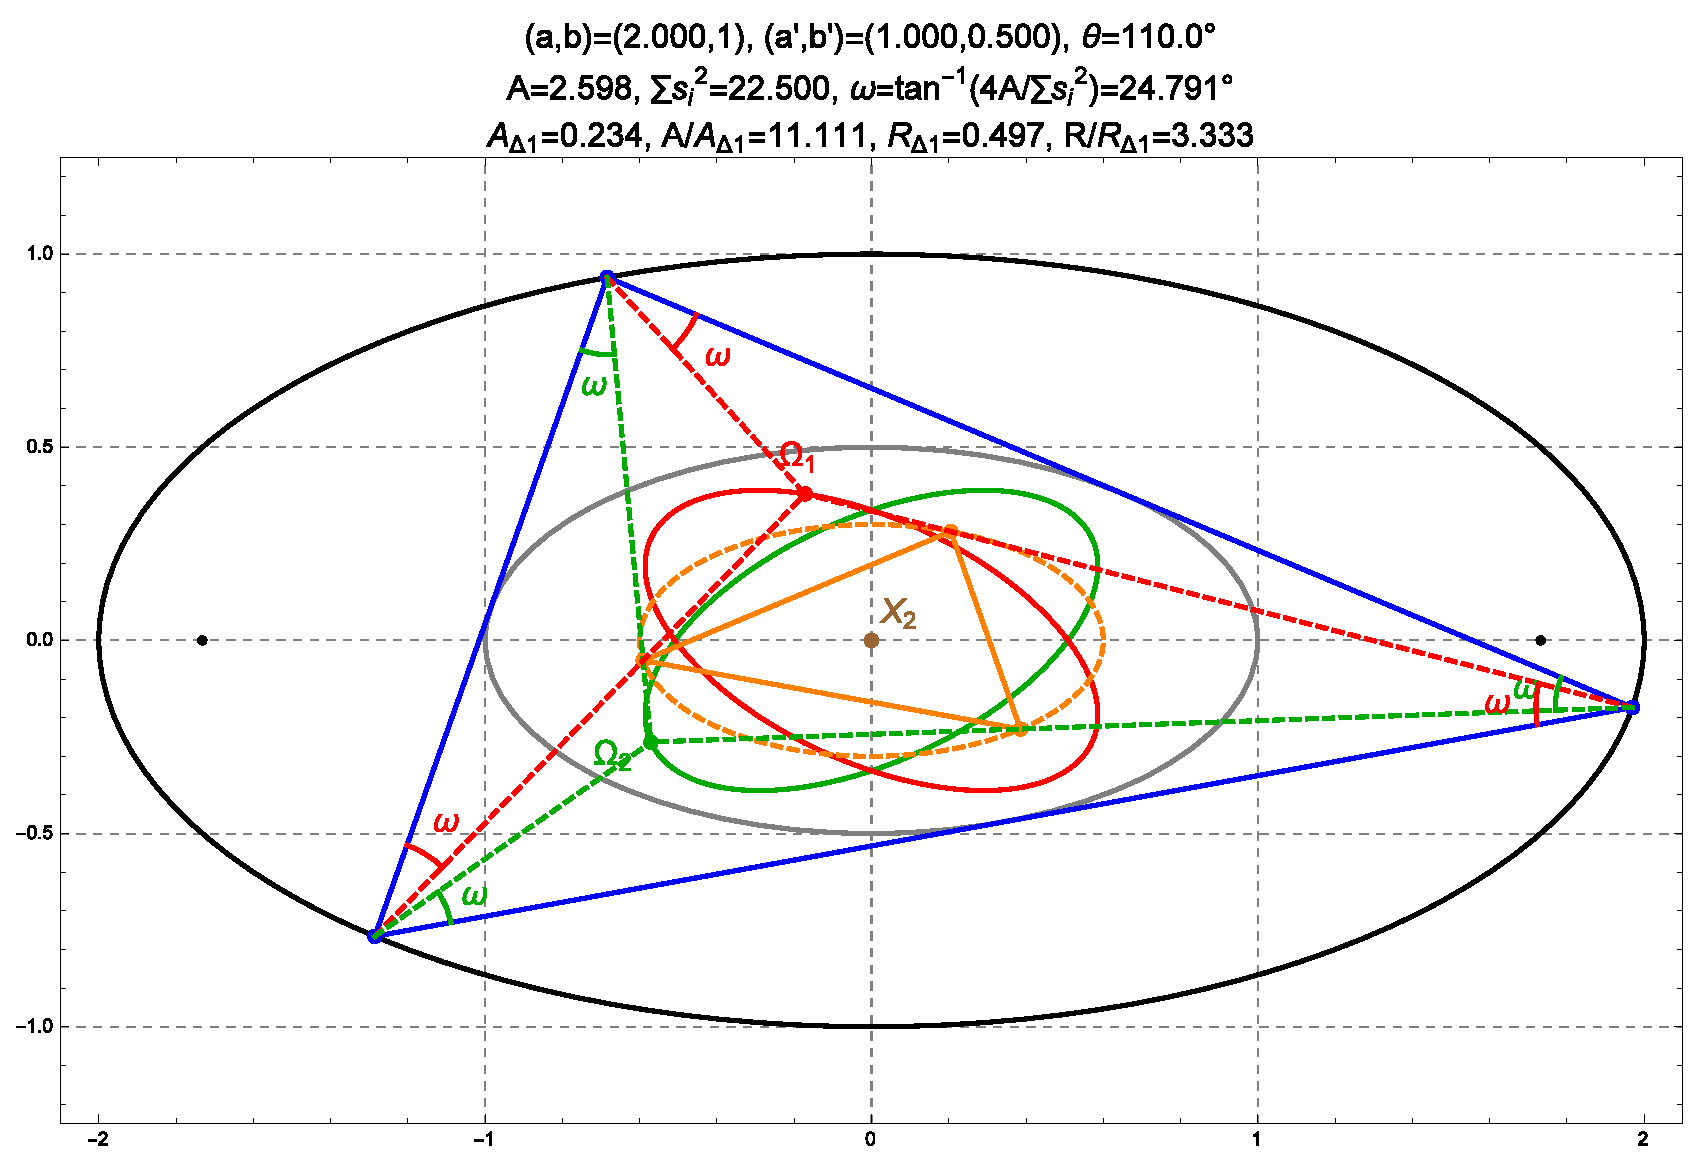
\includegraphics[width=\textwidth]{pics_06_060_first_brocard_tri_locus.eps}
\caption{Over homothetic 3-periodics, the loci of the two Brocard points $\Omega_1$ and $\Omega_2$ are tilted ellipses (red and green) of aspect ratio equal to those in the pair, see \href{https://youtu.be/2fvGd8wioZY}{Video}. Also shown (dashed orange) is the locus of the vertices of the first Brocard triangle (orange): this is an axis-aligned ellipse also homothetic to the pair.\href{https://youtu.be/13i3JGY-fK4}{Video}, \href{https://bit.ly/3iaISog}{Live}}
\label{fig:06-homot-loci}
\end{figure}

Referring to Figure~\ref{fig:06-homot-loci}:

\begin{proposition}
Over homothetic 3-periodics, the loci of the Brocard points $\Omega_1$ and $\Omega_2$ are ellipses $\E_1$ and $\E_2$ which modulo rotation are homothetic to the ellipses in the pair. The loci are reflected images of each other about either the $x$ or $y$ axis.
\end{proposition}

\begin{proof}
The loci are given by
	
	\[\E_1(x,y)= {\frac { \left( 7\,{a}^{4}+6\,{a}^{2}{b}^{2}+3\,{b}^{4} \right) {x}^{2
}}{{a}^{2} \left( a^2-b^2 \right) ^{2}   }}+{\frac {
 \left( 3\,{a}^{4}+6\,{a}^{2}{b}^{2}+7\,{b}^{4} \right) {y}^{2}}{{b}^{
2} \left( {a}^{2}-  {b}^{2} \right)^2 }}- \,{\frac {
4\sqrt {3} \left( {a}^{2}+{b}^{2} \right) xy}{ab \left( {a}^{2}-{b}^{2}
 \right) }}-1
	\]
	\[\E_2(x,y)=	 {\frac { \left( 7\,{a}^{4}+6\,{a}^{2}{b}^{2}+3\,{b}^{4} \right) {x}^{2
}}{{a}^{2} \left( a^2-b^2 \right) ^{2}   }}+{\frac {
 \left( 3\,{a}^{4}+6\,{a}^{2}{b}^{2}+7\,{b}^{4} \right) {y}^{2}}{{b}^{
2} \left( {a}^{2}- {b}^{2} \right)^2 }}+ \,{\frac {
4\sqrt {3} \left( {a}^{2}+{b}^{2} \right) xy}{ab \left( {a}^{2}-{b}^{2}
 \right) }}-1
\]	
	The angle $\theta$ between the axes of ellipses $\E_1$  and $\E_2$ is given by
	\[\tan\theta = \frac{4\sqrt{3}(a^2+b^2) ab}{3a^4+2a^2b^2+3b^4}.\]
\end{proof}

In no other CAP family so far studied, is the locus of either Brocard point an ellipse. This informs:

\begin{conjecture}
Over 3-periodics in a CAP family, the locus of the Brocard points is an ellipse if and only if the ellipses are homothetic.
\label{conj:06-homoth-broc-loci}
\end{conjecture}

